\begin{table}[h!]
  \centering
  \caption{Descriptive Statistics and Correlations}
  \label{tab:descriptives}
  % GENERATED by analysis/descriptives.py -- do not edit.
%
% Rows only. The float, caption and label live in
% chapters/98_TablesFigures.tex, per the guideline that tables sit
% after the references, one per page.
%
% Correlations carry no significance markers ON PURPOSE. The 480
% observations are nested (12 per question, 40 per condition), so the
% independence assumption behind a significance test does not hold.
% Do not add stars.
\setlength{\tabcolsep}{3pt}
\footnotesize
\begin{tabular}{@{}lrrrrrrrrrrr@{}}
\toprule
Variable & \multicolumn{1}{c}{$M$} & \multicolumn{1}{c}{$SD$} & \multicolumn{1}{c}{1} & \multicolumn{1}{c}{2} & \multicolumn{1}{c}{3} & \multicolumn{1}{c}{4} & \multicolumn{1}{c}{5} & \multicolumn{1}{c}{6} & \multicolumn{1}{c}{7} & \multicolumn{1}{c}{8} & \multicolumn{1}{c}{9} \\
\midrule
1. Chunk size (500 vs.\ 200) & 0.500 & 0.501 &  &  &  &  &  &  &  &  &  \\
2. Retrieval strategy: BM25 & 0.333 & 0.472 & .00 &  &  &  &  &  &  &  &  \\
3. Retrieval strategy: hybrid & 0.333 & 0.472 & .00 & $-$.50 &  &  &  &  &  &  &  \\
4. Indexing: metadata-enriched & 0.500 & 0.501 & .00 & .00 & .00 &  &  &  &  &  &  \\
5. Question category: thematic & 0.375 & 0.485 & .00 & .00 & .00 & .00 &  &  &  &  &  \\
6. Question category: comparative & 0.275 & 0.447 & .00 & .00 & .00 & .00 & $-$.48 &  &  &  &  \\
7. Number of gold anchors & 1.850 & 0.727 & .00 & .00 & .00 & .00 & .73 & .13 &  &  &  \\
8. Chunk-size-sensitive anchor & 0.175 & 0.380 & .00 & .00 & .00 & .00 & .05 & .01 & .00 &  &  \\
9. Anchor coverage@5 & 0.228 & 0.371 & $-$.02 & $-$.10 & .07 & .27 & $-$.31 & $-$.06 & $-$.41 & .03 &  \\
10. MRR@5 & 0.147 & 0.287 & .00 & $-$.14 & .10 & .25 & $-$.28 & $-$.06 & $-$.36 & $-$.02 & .85 \\
\bottomrule
\end{tabular}
\normalsize

  \floatfoot{\emph{Note.} $N = 480$ observations, comprising \thesisNumQuestionsScored{}
    benchmark questions crossed with \thesisNumConditions{} retrieval
    conditions. The \thesisNumQuestionsUnanswerable{} unanswerable benchmark
    items are excluded from both retrieval metrics -- they have no gold anchor
    to retrieve -- so the question count here is
    \thesisNumQuestionsScored{}, not the \thesisNumQuestions{} items in the
    benchmark. Dichotomous variables are
    coded 0/1. Retrieval strategy enters as indicators for BM25 and hybrid, and
    question category as indicators for thematic and comparative; dense and
    factual are carried implicitly and are not reference levels. Each
    indicator's correlation therefore contrasts the level it names against all
    the others pooled. The design factors correlate .00 with one another,
    reflecting the balance of the fully crossed grid rather than a finding; the
    $-$.50 between the BM25 and hybrid indicators and the $-$.48 between the
    thematic and comparative indicators are structural.
    Correlations are Pearson coefficients; for a dichotomous variable this is
    the point-biserial correlation, and for two dichotomous variables the phi
    coefficient. The observations are nested -- \thesisNumConditions{} share
    each question and \thesisNumQuestionsScored{} share each condition -- so the
    independence assumption behind a significance test does not hold. Both
    outcomes are also concentrated at zero: anchor coverage@5 is exactly zero on
    69.4\% of the 480 observations, and MRR@5 is zero on the same ones, since
    coverage is zero exactly when no anchor has a defined rank. Pearson's
    estimate survives non-normality; the significance test built on it does
    not. No $p$ values or significance markers are
    reported: read these coefficients as descriptive of this sample rather than
    confirmatory. Anchor count is largely determined by question category
    because the question type is the evidence requirement: a factual question
    asks for one figure and carries one anchor, a comparative question cannot be
    answered from one side and carries one anchor per company, and a thematic
    question carries two or three. The number of transcripts a question spans is
    equal to its anchor count on all \thesisNumQuestionsScored{} questions and
    is therefore not listed separately.}
\end{table}

\newpage

\begin{table}[h!]
  \centering
  \caption{Retrieval Quality by Condition}
  \label{tab:retrieval-metrics}
  % GENERATED by scripts/build_thesis_macros.py -- do not edit.
% Stage 1 is generator-independent: these numbers are identical under
% every generator arm, because retrieval never calls one.
%
% NOTE the source column name: 'overall_not_cross_category_comparable'.
% The overall figure pools categories with different achievable ceilings,
% so it is NOT comparable across categories. Use the per-category
% breakdown for any cross-category claim.
\begin{tabular}{llrr}
\toprule
Chunk size & Retrieval strategy & Anchor coverage@5 & MRR@5 \\
\midrule
\multicolumn{4}{l}{\emph{Text-only}} \\
200 & Dense & .083 & .043 \\
200 & BM25 & .125 & .064 \\
200 & Hybrid & .163 & .090 \\
500 & Dense & .113 & .073 \\
500 & BM25 & .138 & .074 \\
500 & Hybrid & .138 & .109 \\
\midrule
\multicolumn{4}{l}{\emph{Metadata-enriched}} \\
200 & Dense & .408 & .241 \\
200 & BM25 & .237 & .153 \\
200 & Hybrid & .392 & .290 \\
500 & Dense & .375 & .290 \\
500 & BM25 & .200 & .077 \\
500 & Hybrid & .362 & .260 \\
\bottomrule
\end{tabular}

  \floatfoot{\emph{Note.} Anchor coverage@5 and MRR@5 over the \thesisNumQuestionsScored{}
    retrieval-scored benchmark questions, by chunk size, retrieval strategy, and
    indexing representation. Stage~1 is generator-independent: retrieval never
    calls a generator, so these values are identical under every generator
    arm. The \thesisNumQuestionsUnanswerable{} unanswerable items are excluded
    from both metrics, since they have no gold anchor to retrieve. Anchor coverage@5 is the fraction of a question's own
    gold anchors found in the top~5, not textbook Recall@5. Values print to three decimals and, being bounded by 1, carry no leading zero. Hybrid retrieval at 200 tokens and dense retrieval at 500 tokens print alike on MRR@5 but are not tied: hybrid is the larger. Differences and gaps quoted in the text and in Figure~\ref{fig:coverage} are computed on the unrounded values.}
\end{table}

\newpage

\begin{table}[h!]
  \centering
  \caption{Paired Comparisons of Retrieval Quality}
  \label{tab:stage1-tests}
  \footnotesize
  \renewcommand{\arraystretch}{0.9}
  \begin{tabular}{@{}lrrrrrr@{}}
  \toprule
  & \multicolumn{3}{c}{Anchor coverage@5} & \multicolumn{3}{c}{MRR@5} \\
  \cmidrule(lr){2-4} \cmidrule(l){5-7}
  Comparison & W--L & $p$ & $|r|$ & W--L & $p$ & $|r|$ \\
  \midrule
  \multicolumn{7}{@{}l}{\textbf{Panel A: All questions, pairs differing in one factor}} \\
  \multicolumn{7}{@{}l}{\emph{Family 1: metadata-enriched against text-only}} \\
  Dense, 200 & 17--1 & .001 & .862 & 19--3 & .003 & .741 \\
  BM25, 200 & 6--1 & .075 &  & 8--2 & .049 & .709 \\
  Hybrid, 200 & 12--1 & .009 & .824 & 17--3 & .011 & .668 \\
  Dense, 500 & 12--0 & .006 & .883 & 14--2 & .007 & .795 \\
  BM25, 500 & 5--3 & .248 &  & 5--4 & .720 &  \\
  Hybrid, 500 & 12--2 & .010 & .763 & 13--3 & .021 & .672 \\
  \multicolumn{7}{@{}l}{\emph{Family 2: within text-only}} \\
  Dense, 200 vs 500 & 3--6 & 1.000 &  & 3--8 & 1.000 & .456 \\
  BM25, 200 vs 500 & 3--4 & 1.000 &  & 4--4 & 1.000 &  \\
  Hybrid, 200 vs 500 & 3--3 & 1.000 &  & 4--7 & 1.000 & .241 \\
  BM25 vs dense, 200 & 4--2 & 1.000 &  & 6--3 & 1.000 &  \\
  BM25 vs hybrid, 200 & 1--3 & 1.000 &  & 3--5 & 1.000 &  \\
  Dense vs hybrid, 200 & 1--5 & .651 &  & 1--8 & .225 &  \\
  BM25 vs dense, 500 & 4--4 & 1.000 &  & 5--6 & 1.000 & .107 \\
  BM25 vs hybrid, 500 & 3--4 & 1.000 &  & 3--8 & 1.000 & .456 \\
  Dense vs hybrid, 500 & 2--3 & 1.000 &  & 3--5 & 1.000 &  \\
  \multicolumn{7}{@{}l}{\emph{Family 3: within metadata-enriched}} \\
  Dense, 200 vs 500 & 4--2 & 1.000 &  & 7--11 & 1.000 & .262 \\
  BM25, 200 vs 500 & 5--3 & 1.000 &  & 7--6 & 1.000 & .320 \\
  Hybrid, 200 vs 500 & 5--4 & 1.000 &  & 9--9 & 1.000 & .103 \\
  BM25 vs dense, 200 & 2--12 & .249 & .604 & 6--16 & .947 & .332 \\
  BM25 vs hybrid, 200 & 1--9 & .364 & .645 & 2--14 & .078 & .679 \\
  Dense vs hybrid, 200 & 4--3 & 1.000 &  & 7--11 & 1.000 & .216 \\
  BM25 vs dense, 500 & 2--11 & .249 & .620 & 3--17 & .032 & .676 \\
  BM25 vs hybrid, 500 & 0--9 & .080 &  & 0--17 & .004 & .878 \\
  Dense vs hybrid, 500 & 3--3 & 1.000 &  & 7--7 & 1.000 & .151 \\
  \bottomrule
  \end{tabular}
\end{table}

\newpage

\begin{table}[h!]
  \ContinuedFloat
  \centering
  \caption[]{Paired Comparisons of Retrieval Quality (Continued)}
  \footnotesize
  \renewcommand{\arraystretch}{0.9}
  \begin{tabular}{@{}lrrrrrr@{}}
  \toprule
  & \multicolumn{3}{c}{Anchor coverage@5} & \multicolumn{3}{c}{MRR@5} \\
  \cmidrule(lr){2-4} \cmidrule(l){5-7}
  Comparison & W--L & $p$ & $|r|$ & W--L & $p$ & $|r|$ \\
  \midrule
  \multicolumn{7}{@{}l}{\textbf{Panel B: Family 1 by question category}} \\
  \multicolumn{7}{@{}l}{\emph{Factual}} \\
  Dense, 200 & 9--0 & .016 &  & 10--1 & .048 & .724 \\
  BM25, 200 & 4--0 & .091 &  & 5--0 & .079 &  \\
  Hybrid, 200 & 7--0 & .024 &  & 9--1 & .042 & .790 \\
  Dense, 500 & 9--0 & .016 &  & 10--0 & .021 & .886 \\
  BM25, 500 & 4--1 & .180 &  & 4--2 & .666 &  \\
  Hybrid, 500 & 8--0 & .019 &  & 9--0 & .035 &  \\
  \multicolumn{7}{@{}l}{\emph{Thematic}} \\
  Dense, 200 & 2--1 & 1.000 &  & 2--2 & 1.000 &  \\
  BM25, 200 & 0--1 & 1.000 &  & 0--2 & .899 &  \\
  Hybrid, 200 & 2--1 & 1.000 &  & 2--2 & 1.000 &  \\
  Dense, 500 & 1--0 & 1.000 &  & 1--2 & 1.000 &  \\
  BM25, 500 & 0--0 & n/t &  & 0--0 & n/t &  \\
  Hybrid, 500 & 2--1 & 1.000 &  & 2--2 & 1.000 &  \\
  \multicolumn{7}{@{}l}{\emph{Comparative}} \\
  Dense, 200 & 6--0 & .188 &  & 7--0 & .094 &  \\
  BM25, 200 & 2--0 & 1.000 &  & 3--0 & 1.000 &  \\
  Hybrid, 200 & 3--0 & 1.000 &  & 6--0 & .156 &  \\
  Dense, 500 & 2--0 & 1.000 &  & 3--0 & 1.000 &  \\
  BM25, 500 & 1--2 & 1.000 &  & 1--2 & 1.000 &  \\
  Hybrid, 500 & 2--1 & 1.000 &  & 2--1 & 1.000 &  \\
  \midrule
  \multicolumn{7}{@{}l}{\textbf{Panel C: Families 2 and 3 by question category}} \\
  & Testable & Min.\ $p$ & & Testable & Min.\ $p$ & \\
  Family 2, factual & 15 of 15 & 1.000 & & 15 of 15 & 1.000 & \\
  Family 2, thematic & 15 of 15 & 1.000 & & 15 of 15 & 1.000 & \\
  Family 2, comparative & 14 of 15 & 1.000 & & 15 of 15 & 1.000 & \\
  Family 3, factual & 14 of 15 & .355 & & 15 of 15 & .071 & \\
  Family 3, thematic & 13 of 15 & 1.000 & & 15 of 15 & .950 & \\
  Family 3, comparative & 15 of 15 & 1.000 & & 15 of 15 & 1.000 & \\
  \bottomrule
  \end{tabular}
  \floatfoot{\emph{Note.} Two-sided paired Wilcoxon signed-rank tests over the
    \thesisNumQuestionsScored{} retrieval-scored questions
    (\thesisNumQuestionsFactual{} factual, \thesisNumQuestionsThematic{}
    thematic, \thesisNumQuestionsComparative{} comparative). Condition labels
    give retrieval strategy and chunk size in tokens. W--L counts the questions
    on which the first-named condition scored higher and lower; the rest tied.
    $p$ is Holm-adjusted within the family, separately for each metric and each
    scope. $|r|$ is the magnitude of $r = z / \sqrt{n_{\neq 0}}$, printed only
    where 10 or more questions were untied; its sign is an artifact of the
    statistic, so direction is read from W--L. n/t: every question tied, so no
    test was run and no Holm rank was used. Families 2 and 3 hold all 15
    pairwise comparisons within one representation, and H1 and H2 share them,
    so each was corrected once. Panel~A lists only the nine pairs per family
    that differ in chunk size alone or in strategy alone; the six that differ
    in both isolate neither factor and are not shown, and one of them is
    significant on metadata-enriched MRR@5. Panel~C gives, for each category
    block, how many of the 15 comparisons were testable and the smallest
    adjusted $p$ among them, over all 15 pairs. Every testable comparison of a
    pair differing in chunk size alone returned 1.000 in every block of both
    families.}
\end{table}

\newpage

\begin{table}[h!]
  \centering
  \caption{Answer Outcomes by Ground-Truth Case}
  \label{tab:case-outcome}
  % GENERATED by scripts/build_thesis_macros.py from qwen3.8-27b@q8_k_xl -- do not edit.
%
% Rows only. The float, caption and label live in
% chapters/98_TablesFigures.tex, per the guideline that tables sit
% after the references, one per page.
%
% INTERPRET PER CASE. Different cases have different achievable
% outcomes -- answered_grounded_correct is impossible in Case A by
% construction, since unanswerable items carry no transcript_ids and
% the on-target test cannot pass -- so a pooled RATE averages away the
% exact distinction this table exists for.
%
% The Total row below is a RECONCILIATION, not a result: it shows the
% four outcomes account for every generation. Do not compute a rate,
% share or comparison on it. (This block used to read NEVER POOLED,
% which the table contradicted by carrying its own Total row;
% corrected 2026-09-09 to match the Methods wording.)
%
% `grounded, off target` is NOT an answer-quality column. It says no
% supporting chunk belonged to the question's own transcript_ids,
% which is a fact about retrieval targeting.
\begin{tabular}{@{}lrrrrr@{}}
\toprule
Case & \multicolumn{1}{c}{\shortstack[c]{abstained}} & \multicolumn{1}{c}{\shortstack[c]{grounded,\\on target}} & \multicolumn{1}{c}{\shortstack[c]{grounded,\\off target}} & \multicolumn{1}{c}{\shortstack[c]{ungrounded}} & \multicolumn{1}{c}{$n$} \\
\midrule
A & 55 & 0 & 1 & 4 & 60 \\
B & 195 & 25 & 109 & 4 & 333 \\
C & 35 & 109 & 2 & 1 & 147 \\
\midrule
Total & 285 & 134 & 112 & 9 & 540 \\
\bottomrule
\end{tabular}

  \floatfoot{\emph{Note.} All \thesisNumConditions{} conditions pooled,
    $n = \thesisQeightNumRecords{}$ generations from
    \thesisQeightModel{}. Case~A: no gold anchor exists in the corpus
    (the \thesisNumQuestionsUnanswerable{} unanswerable items). Case~B:
    answerable, but no gold anchor appeared in the top~\thesisTopK{}.
    Case~C: at least one gold anchor appeared. Correct behavior is
    abstention in Cases~A and~B and a grounded, on-target answer in
    Case~C. Cases are computed from Stage~1 retrieval and are therefore
    identical under every generator. \emph{Grounded, on target} means
    every numeric claim appears verbatim in a retrieved chunk and at
    least one supporting chunk belongs to the question's own
    transcripts; \emph{grounded, off target} means the claims trace to
    retrieved text but none of the supporting chunks does. The latter is
    a statement about retrieval targeting, not about answer quality.
    Grounding is a verbatim-substring proxy and is deliberately
    conservative: a figure restated in different units reads as
    unsupported.}
\end{table}

\newpage

\begin{table}[h!]
  \centering
  \caption{Case~C Conversion by Anchor Coverage}
  \label{tab:coverage-split}
  \footnotesize
  \begin{tabular}{@{}llrrrrrr@{}}
  \toprule
  & & \multicolumn{3}{c}{Converted / $n$} & \multicolumn{3}{c}{Not converted, pooled} \\
  \cmidrule(lr){3-5} \cmidrule(l){6-8}
  Category & Coverage & Text-only & Enriched & Pooled & Abstained & Off target & Ungrounded \\
  \midrule
  Thematic & Partial & 13/13 & 14/16 & 27/29 (93.1\%) & 1 & 1 & 0 \\
  Thematic & Full & -- & -- & -- & -- & -- & -- \\
  \midrule
  Comparative & Partial & 3/18 & 8/28 & 11/46 (23.9\%) & 33 (71.7\%) & 1 & 1 \\
  Comparative & Full & -- & 2/2 & 2/2 & 0 & 0 & 0 \\
  \bottomrule
  \end{tabular}
  \floatfoot{\emph{Note.} Case~C observations of \thesisQeightModel{} with two or more gold
    anchors, all \thesisNumConditions{} conditions. Partial coverage: some but
    not all of a question's anchors in the top~\thesisTopK{}; full: all of them.
    Thematic questions carry two or three anchors and comparative questions
    two, one per company. No thematic observation reached full coverage. The
    comparative full-coverage cell rests on two observations. Converted means
    answered grounded and on target; the last three columns account for the
    remaining pooled observations. Off target describes retrieval targeting,
    not answer quality. The figures have no reference values to be validated
    against and are reported as computed and unchecked.}
\end{table}

\newpage

\begin{table}[h!]
  \centering
  \caption{Categories From the Manual Faithfulness Review}
  \label{tab:review-categories}
  \begin{tabularx}{\textwidth}{@{}lXr@{}}
  \toprule
  Code & Description & Items \\
  \midrule
  \multicolumn{3}{@{}l}{\emph{Panel A: Generator behaviors}} \\
  P1 & Gives one company's material under another company's name & 12 \\
  P2 & Declines the whole question when the context holds one side of it & 8 \\
  P3 & Dates material to a period it does not come from & 3 \\
  P4 & Answers from outside the asked window, but says so & 2 \\
  \midrule
  \multicolumn{3}{@{}l}{\emph{Panel B: Instrument findings}} \\
  I1 & A correctly read date is checked as though it were a figure & 2 \\
  I2 & Arithmetic the answer itself marks as derived counts as ungrounded & 1 \\
  I3 & The verbatim fallback cannot match a faithful paraphrase & 1 \\
  I4 & The off-target label reflects retrieval targeting, not answer quality & 12 \\
  I5 & A gold anchor does not answer its own question & 1 \\
  I6 & The same failure receives two different labels & 1 \\
  \bottomrule
  \end{tabularx}
  \floatfoot{\emph{Note.} Items are generations of \thesisQeightModel{} read in the manual
    review, $n = \thesisNumReviewItems{}$. Panel~A and Panel~B are separate
    axes, one about the generator and one about the scoring instrument and
    benchmark, and are not one list. Both are inductive and post hoc: they were
    named in a second pass, after every item had been read, and the first pass
    proposed no groupings. In Panel~A, two items each carry two
    behaviors, so the 25 assignments cover 23 items; the other 25 items carry
    none. In Panel~B, I1 is a traced defect in the outcome classifier,
    reported and not corrected; I2 and I3 are not defects but the conservative
    grounding proxy behaving as specified. I4's count is 12 of the 17
    off-target records drawn into the review, out of
    \thesisQeightAnsweredGroundedOfftarget{} in the grid: a proportion within
    a sample, not extrapolated to the grid. I5 is \texttt{ref\_fact\_14},
    reviewed under \texttt{chunk200\_bm25\_enriched}: its gold anchor is a three-year cumulative figure while its reference answer drops that scope, so an answer that reports the figure correctly, as a three-year figure, does not match the reference, and the item cannot score a correct answer as correct.
    The defect is also recorded in the benchmark documentation (\texttt{benchmark\_process.md}, Section~10.6).
    Check~3, an automatic diagnostic outside the review, flags a record labeled
    grounded and on target when a substantive figure in it is supported only by
    chunks from outside the question's own transcripts. On the matched subset,
    the items in Case~C under both representations, it flagged 5 of the 24
    converted under text-only (20.8\%) and 7 of the 29 converted under
    metadata-enriched (24.1\%); on the 22 converted under both, it flagged 4 of
    22 (18.2\%) under text-only and 7 of 22 (31.8\%) under metadata-enriched,
    the same seven records, none of them among the seven that converted under
    metadata-enriched alone.}
\end{table}

\newpage

\begin{table}[h!]
  \centering
  \caption{Robustness Check Against a Second Generator}
  \label{tab:robustness}
  \begin{tabular}{@{}lrr@{}}
  \toprule
  \multicolumn{3}{@{}l}{\textbf{Panel A: Outcome-label agreement}} \\
  & Disagreements & $n$ \\
  \midrule
  \multicolumn{3}{@{}l}{\emph{By question category}} \\
  Factual & 1 & 168 \\
  Thematic & 24 & 180 \\
  Comparative & 12 & 132 \\
  Unanswerable & 5 & 60 \\
  \multicolumn{3}{@{}l}{\emph{By case}} \\
  Case~A & 5 & 60 \\
  Case~B & 27 & 333 \\
  Case~C & 10 & 147 \\
  \midrule
  All records & 42 & 540 \\
  \bottomrule
  \end{tabular}

  \vspace{1.5em}

  \begin{tabular}{@{}lrr@{}}
  \toprule
  \multicolumn{3}{@{}l}{\textbf{Panel B: Replication}} \\
  & Reported arm & Robustness arm \\
  \midrule
  Case~C conversion & \thesisQeightCaseCConversion{} (\thesisQeightCaseCConversionPct{})
    & \thesisFlashRobustnessCaseCConversion{} (\thesisFlashRobustnessCaseCConversionPct{}) \\
  Thematic, partial coverage & 27/29 & 27/29 \\
  Comparative, partial coverage & 11/46 & 14/46 \\
  Matched subset, text-only & 24/38 & 23/38 \\
  Matched subset, enriched & 29/38 & 33/38 \\
  Grounded, on target (grid) & \thesisQeightAnsweredGroundedCorrect{}
    & \thesisFlashRobustnessAnsweredGroundedCorrect{} \\
  Grounded, off target (grid) & \thesisQeightAnsweredGroundedOfftarget{}
    & \thesisFlashRobustnessAnsweredGroundedOfftarget{} \\
  \bottomrule
  \end{tabular}
  \floatfoot{\emph{Note.} Reported arm: \thesisQeightModel{}. Robustness arm:
    \thesisFlashRobustnessModel{}. Both ran all \thesisNumConditions{}
    conditions, $n = 540$ records each, on the same seed, temperature, and
    prompt hash; the case partition is identical because cases come from
    Stage~1 retrieval. Panel~A compares the outcome label each arm received on
    the same condition and question; the two arms agree on 498 of 540 records
    (92.2\%). The five unanswerable disagreements all come from
    \texttt{ref\_unans\_01} and follow from the robustness arm naming no
    company, so 37 of the 42 are informative. Panel~B: conversion means
    answered grounded and on target; coverage rows are Case~C observations at
    partial coverage, both representations pooled; matched-subset rows are the
    38 items in Case~C under both representations; grid rows count labels over
    all 540 records. The generators differ on several dimensions at once, and
    no difference is attributed to any one of them.}
\end{table}

\newpage

\begin{figure}[h!]
  \centering
  \caption{The Research Model}
  \label{fig:research-model}
  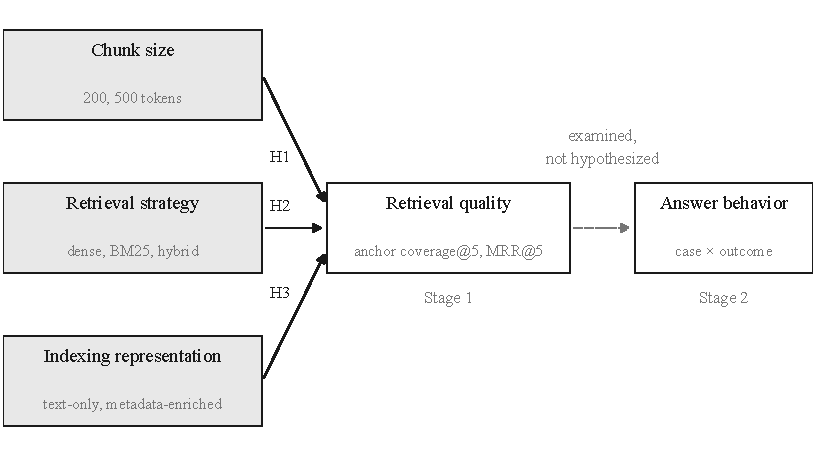
\includegraphics[width=0.92\textwidth]{generated/figure_research_model}
  \floatfoot{\emph{Note.} The three manipulated factors, the retrieval quality
    they are hypothesized to move, and the answer behavior measured beyond it.
    H1 to H3 are stated in Theory, each closing its own derivation. The corpus,
    the questions, the prompt, the generator, the top~\thesisTopK{} retrieved
    chunks, the embedding model, the random seed, and the decoding temperature
    are held constant across all \thesisNumConditions{} conditions. The dashed
    link was examined without a hypothesis being scored on it: at the
    discordant-pair counts these data produce, the exact test's smallest
    attainable \emph{p} value sits above any conventional threshold. Stage~1
    never calls a generator, so its values are identical under every
    generator arm.}
\end{figure}

\newpage

\begin{figure}[h!]
  \centering
  \caption{Effect of Indexing Representation on Retrieval Coverage}
  \label{fig:coverage}
  
\includegraphics[width=0.92\textwidth]{generated/figure_coverage}
  \floatfoot{\emph{Note.} Anchor coverage@5 for each chunk-size and retrieval-strategy
    combination under both indexing representations, over the
    \thesisNumQuestionsScored{} retrieval-scored benchmark questions. The connector length is the change;
    the value beside each pair is that change in coverage points. Stage~1 is
    generator-independent, so these values hold for every generator arm.
    \emph{Movement in this figure is not by itself a significance claim.} On
    Holm-adjusted paired Wilcoxon tests within the six-pair representation
    family, the four dense and hybrid pairs are significant on anchor
    coverage@5 ($p \leq .010$) and the two BM25 pairs are not ($p = .075$ and
    $p = .248$). BM25 at \thesisChunkSizeSmall{} tokens \emph{is} significant on
    MRR@5 ($p = .049$), which this figure does not show.}
\end{figure}

\newpage

\begin{figure}[h!]
  \centering
  \caption{Answer Outcomes by Ground-Truth Case}
  \label{fig:case-outcome}
  
\includegraphics[width=0.92\textwidth]{generated/figure_case_outcome}
  \floatfoot{\emph{Note.} Share of generations falling to each outcome within each case, all
    \thesisNumConditions{} conditions pooled, $n = \thesisQeightNumRecords{}$
    from \thesisQeightModel{}. Counts are printed inside each segment; segments
    below seven percent are left unlabeled and their counts are in
    Table~\ref{tab:case-outcome}. The three cases are shown as shares rather
    than counts because their sizes differ by an order of magnitude, and the
    point is that the three have different \emph{shapes} -- which is why
    outcomes are interpreted per case rather than pooled. The cases differ in
    which outcomes are achievable at all -- one outcome is impossible in
    Case~A by construction -- so a pooled rate would average away the
    distinction the scheme exists to preserve. Pooled column totals are
    reported in Table~\ref{tab:case-outcome}, but only as a reconciliation
    that the four outcomes account for every generation; no rate, share, or
    comparison is computed on them. \emph{Grounded, off target} means no
    supporting chunk belonged to the question's own transcripts; it describes
    retrieval targeting, not answer quality.}
\end{figure}
